\documentclass{standalone}
\usepackage{tikz}
\usepackage{ctex,siunitx}
\usepackage{tkz-euclide}
\usepackage{amsmath}
\usetikzlibrary{patterns, calc}
\usetikzlibrary {decorations.pathmorphing, decorations.pathreplacing, decorations.shapes,}
\begin{document}
\small
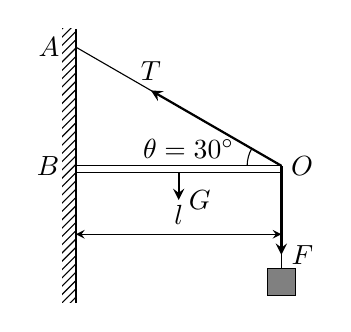
\begin{tikzpicture}[>=stealth,scale=0.87]
  \fill [pattern=north east lines](-2.2,-2) rectangle (-2,2);
  \draw [thick](-2,2)--(-2,-2);
  \draw (-2,-0.1)rectangle (1,0);
  \draw (1,0) node[right]{$O$}--(-2,1.732);
  \draw[->, thick](1,0)--++(150:2.2)node[above]{$T$};
  \draw (1,0)--(1,-1.5);
  \draw[->, thick] (1,0)--(1,-1.3) node [right]{$F$};
  \draw [fill=gray](1-.2,-1.5-.4) rectangle (1+.2, -1.5);
  \draw[<->] (-2,-1.0) -- node[above]{$l$} (1,-1.0);
  \draw [thick,->] (-.5, -.1)--(-.5,-.5)node[right]{$G$};
  \node at (-2.1,1.732) [left]{$A$};
  \node at (-2.1,0) [left]{$B$};
  \draw (.5,0) arc (180:150:.5)node[left=1mm]{$\theta = \ang{30}$};
\end{tikzpicture}
\end{document}